\section{Sprint 4 conclusion}\label{sec:sprint4conclusion}
This section concludes sprint 4 and will summarize the progress that has been made on the game and discuss the retrospective meeting conducted at the end of sprint 4.

\subsection{Current product}
In \autoref{fig:sprint-4-state-of-game} the two current states of the game can be seen.
We are currently able to connect to the host in the lobby, as seen on \autoref{fig:sprint-4-lobby}, which will lead to \autoref{fig:sprint-4-game} when the host has started the game.
\begin{figure}[H]
    \centering
    \begin{subfigure}{.5\textwidth}
        \centering
        
\includegraphics[width=1\linewidth]{figures/sprint-4-lobby.PNG}
        \caption{The lobby where you need to input the IP address to connect.}
        \label{fig:sprint-4-lobby}
    \end{subfigure}
    \begin{subfigure}{.4\textwidth}
        \centering
        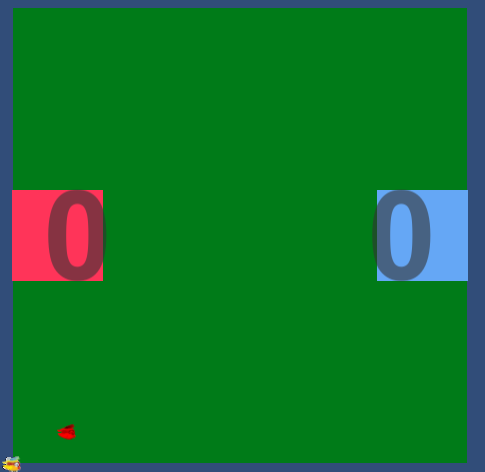
\includegraphics[width=.8\linewidth]{figures/sprint-4-game.PNG}
        \caption{The current playing field with goal zones, goal score and players.}
        \label{fig:sprint-4-game}
    \end{subfigure}
    \caption{The current state of the game}
    \label{fig:sprint-4-state-of-game}
\end{figure}

\subsubsection{Pozyx}
There are not a lot of tasks missing with Pozyx, but there are several tasks that needs to be completed in the next sprint to make it work.
\\\\
During the initial test of the program describe in \autoref{sec:initial-test} several exception occurred, which was because that the input data was not correctly formatted.
This should be easy to fix.
In the initial test there were also discovered problems with the firmware, where pozyx would not send positional data to the host, but only send coordinates of 0.0.

\subsubsection{Game}
If the problems with pozyx gets fixed, the game should be working fine.
But in the current iteration of the game, you are unable to win the game.
This is a highly prioritized task on Unity, which we intend to implement in the last sprint.

\subsubsection{Networking}
To be able to win the game, it is necessary for the host signal winning the game to the clients and therefore a package needs to be specified.

\subsection{Retrospective on the process}
This subsection will elaborate the retrospective meeting that was held on the May 12th.

\subsubsection*{How does the process with Jira work?}
The process with Jira will change with the last sprint.
For previous sprints there were a \textit{Suggested} column and \textit{Discussed} column, but in the upcoming sprint the \textit{Discussed} column will no longer be used.
It will either be moved to \textit{Chosen for development} or a \textit{Future work} column that was added.
This sprint will be the last, and therefore we find it less important to prioritize the tasks.
Either the task has to be completed, or it has to be documented in \textit{Future work}.

\subsubsection*{How has pair programming been working?}
Pair programming works well, but there are some challenges with online pair programming in Unity, as it is required to compile to an android device, which is more difficult to share with the other programmer.

\subsubsection*{How is the daily stand-up working?}
When the members of the group does not have a task, the daily stand up seems pointless, as they do not have much to say.
To change this by the start of the day people will have 5 minutes to look at tasks and pick one, so that they have the opportunity to discuss that.
\\\\
There were also a comment that estimations of completed tasks were inaccurate.
So whenever someone said the previous day that they would have completed the task, they have to specify the reasons why they did not complete the tasks.
\\\\
Sometimes it is suspected that the motivation is low, and to help this we will introduce pair report writing.
If people have tried it in the upcoming days, it will be evaluated to see if it is something that is well liked.

\subsubsection*{How are the reviews going?}
The group members are more aware of doing the reviews, so reviews often gets done at the same day or in the morning the next day.

\subsubsection*{Closing comments}
At the end of the sprint retrospective we went through the tasks that was completed in the sprint to see what was interesting to describe in the report.

